\documentclass[12pt]{article}
\usepackage[a4paper,margin=1in]{geometry}
\usepackage{setspace}
\usepackage{booktabs}
\usepackage{graphicx}
\usepackage{amsmath}
\usepackage{amssymb}
\usepackage{amsthm}
\usepackage{float}
\usepackage{tabularx}
\usepackage{array}
\usepackage{xcolor}
\usepackage[
  colorlinks=true,
  linkcolor=blue!50!black,
  citecolor=blue!50!black,
  urlcolor=blue!50!black
]{hyperref}
\usepackage[authoryear,round]{natbib}
\graphicspath{{figures/}}

\newtheorem{proposition}{Proposition}

\title{The Risk-Adjusted Cost of Stablecoins as Payment Instruments\\[0.3em]
\large A short working-paper summary}
\author{
Andres Alonso-Robisco\thanks{Banco de Espa\~na.
Corresponding author: \texttt{andres.alonso@bde.es}.
The views expressed are the sole responsibility of the author and do not
necessarily reflect those of Banco de Espa\~na or the Eurosystem.}
}
\date{\today}

\begin{document}
\maketitle
\onehalfspacing

\begin{abstract}
\noindent Sending a fiat-backed stablecoin costs a fraction of a correspondent-banking payment, but the headline fee understates the cost the sender bears: the holder briefly carries a private-issuer liability exposed to counterparty risk and to secondary-market price dispersion when par convertibility breaks. We price both with a global game and obtain risk premiums of 49 basis points for USDC and 71 for USDT, with inverted compositions. Carried into a corridor-level cost comparison, the stablecoin path is dominated where an upgraded public instant-payment rail already exists, wins where none does, and is absorbed once an upgraded public cross-border rail goes live. The category ``stablecoin'' is too coarse to be the unit of supervision. This note is a short, fast-reading version; the formal model, the calibration mechanics, and the full robustness analysis are in a companion internet appendix.
\end{abstract}

\medskip
\noindent\textbf{Keywords:} stablecoins; retail payments; global games; cross-border payments.
\quad\textbf{JEL:} C63; E42; G21; G23; G28.

\clearpage

\section{The puzzle and what we do}\label{sec:intro}

A retail payment from the United States to Mexico over the SWIFT correspondent network costs about 330 basis points of the amount sent \citep{rpw_q3_2025}; the same payment as a USDT transfer on Tron costs about 37 basis points at USD 400 \citep{tronsave_blog_2026}. This two-order-of-magnitude gap is the empirical basis for the claim that stablecoins are a frontier payment technology. The comparison is incomplete: it sets the \emph{announced} cost of the stablecoin against the \emph{all-in} cost of the incumbent.

A stablecoin sender does not pay only the on-chain fee. The sender holds, however briefly, a private-issuer liability convertible into fiat at par on a best-effort basis, and that promise can fail in two ways. The issuer may lack liquid reserves of sufficient quality to redeem at par (a \emph{counterparty} loss), or the secondary market where unmet redemptions clear may be too thin, so the realised conversion price falls below par when demand to convert is high (a \emph{depeg} loss). The depeg loss is a coordination outcome: when many holders convert at once, primary redemption is exhausted and the secondary price falls, a self-fulfilling run.

This note prices that liability and plugs it into a corridor comparison. The argument runs in three quick steps: (i) \emph{why} a global game is the right tool for the redemption decision; (ii) \emph{what} data discipline the two stablecoins we calibrate; and (iii) \emph{how} the resulting risk-adjusted cost compares with public, incumbent, and fintech payment rails. The headline numbers are a 49-basis-point premium for USDC and 71 for USDT, with inverted compositions (USDC depeg-driven, USDT counterparty-driven); a three-regime ordering of corridors; and the supervisory reading that the stablecoin category is too coarse for a single rule.

\section{Why a global game}\label{sec:global_game_policy}

The redemption decision is strategic, not individual. A holder who expects others to convert at the same time anticipates a worse secondary price, so each holder's best action depends on what the rest do. This is the structure of a global game in the spirit of \citet{morris_shin_1998}, adapted to a dual-channel exit: holders redeem first at the issuer (par, up to liquid reserves $R$), and unmet demand spills into a secondary market of finite, stress-contracting depth. Figure~\ref{fig:gg} shows the coordination structure.

\begin{figure}[H]
\centering
\includegraphics[width=0.92\textwidth]{fig_morris_shin_clock_preview.pdf}
\caption{The redemption problem as a coordination game. Each holder observes the issuer fundamental $\theta$ through a noisy private signal $s_i$ and picks a conversion threshold $s^{*}$ given the aggregate run she expects; the aggregate run is in turn set by the threshold everyone uses. Equilibrium is the unique fixed point $s^{*}$.}\label{fig:gg}
\end{figure}

Holders share a latent issuer fundamental $\theta$ and each sees a noisy signal $s_i=\theta+\sigma\varepsilon_i$. They play threshold strategies (convert if $s_i<s^{*}$), so the mass converting at $\theta$ is $D(\theta;s^{*})=\Phi((s^{*}-\theta)/\sigma)$. The marginal holder at $s^{*}$ is indifferent between converting, with payoff $V_R$ (par on the first $R$ units, the depressed secondary price on the rest), and holding, with payoff $V_H$. The equilibrium threshold is the endogenous fixed point
\begin{equation}\label{eq:fixedpoint}
F(s^{*}) := \mathbb{E}_{\theta\mid s_i=s^{*}}\!\left[V_R(D(\theta;s^{*}))-V_H(\theta)\right]=0,
\end{equation}
where $s^{*}$ enters both as the conditioning signal and through the aggregate mass it induces. This two-way dependence is the run, and it admits no closed form; we solve it numerically. The counterparty loss enters the value of \emph{holding}, $V_H=\theta+\omega-\xi h$, where the issuer hazard $h$ and loss-given-default $\xi$ are taken from market proxies; placed there it lowers the value of holding, raises conversion, and feeds the coordination channel rather than cancelling out.

\subsection{What the model delivers}\label{sub:what_it_delivers}

For each issuer the output is three numbers in basis points: a counterparty component $\ell_C=h\,\xi$, a baseline-regime depeg component $\ell_{D,b}$, and a stress-regime depeg component $\ell_{D,s}$. Their probability-weighted sum is the risk premium added to the on-chain fee,
\begin{equation}\label{eq:total_risk_premium}
\Pi_{\text{risk}} = \ell_C + (1-p_s)\,\ell_{D,b} + p_s\,\ell_{D,s},
\end{equation}
with $p_s$ the stress-regime frequency. The counterparty leg is reduced-form by design; the two depeg legs are the structural output of the global game. A natural question is whether the whole exercise reduces to a run probability times a cost, as a fragility model would deliver \citep{klee_etal_2026_fragility}. It does not, and the reason is quantitative: a counterparty-plus-run benchmark recovers $85\%$ of the USDT premium but misses $54\%$ of USDC's, the baseline-regime secondary-market dispersion that a run-probability framework assigns zero weight. The depeg channel is what makes the fundamentals visible.

\subsection{Two coins, different primitives}\label{sub:not_homogeneous}

The two largest fiat-backed stablecoins are not interchangeable. USDC is backed by short-dated Treasuries and cash at G-SIBs with monthly attestation; USDT holds a heterogeneous mix with attestation-only disclosure and a heavier enforcement record, so its hazard $h$ and loss-given-default $\xi$ are structurally higher. USDT's secondary market is deeper and more concentrated; USDC's is shallower and more atomistic. These map to different parameters, and therefore to different premiums.

\section{Data and calibration}\label{sec:calibration}

We calibrate each issuer to its largest historical depeg episode in hourly secondary-market prices: USDC during the March 2023 Silicon Valley Bank failure (96 stress hours, trough $0.902$, mean absolute depeg $240$ basis points), and USDT during the May 2022 Terra collapse (97 stress hours, trough $0.975$, mean absolute depeg $28$ basis points). Seven parameters (the signal noise $\sigma$, the secondary-market block, and the stress-regime prior) are estimated by weighted moment-matching against six price moments per issuer; the issuer counterparty parameters are fixed externally ($h=0.01,\ \xi=0.20$ for USDC; $h=0.02,\ \xi=0.30$ for USDT). The estimation mechanics and the identification analysis are in the internet appendix.

\subsection{The risk premium}\label{sec:identification}

The calibration delivers $\Pi_{\text{risk}}^{\text{USDC}}=48.9$ and $\Pi_{\text{risk}}^{\text{USDT}}=71.2$ basis points. The compositions are inverted (Table~\ref{tab:decomp}, Figure~\ref{fig:decomp}): USDC's premium is depeg-dominant ($54\%$ baseline depeg, $41\%$ counterparty), USDT's is counterparty-dominant ($84\%$ counterparty, $15\%$ baseline depeg). The same coordination machinery, applied to two issuers with different reserves and secondary venues, returns opposite risk profiles. The stress (run) component is small in both ($5\%$ and $0.4\%$): most of the premium is the counterparty hazard plus ordinary, non-crisis conversion friction, not the tail run.\label{sub:interp}

\begin{table}[H]
\centering
\caption{Risk-premium decomposition, basis points. Compositions are inverted.}\label{tab:decomp}
\begin{tabular}{lrrl}
\toprule
Component & USDC & USDT & Note \\
\midrule
$\ell_C$ counterparty            & 20.0 (41\%) & 60.0 (84\%) & Tether higher $h,\xi$ \\
$\ell_{D,b}$ baseline (weighted) & 26.4 (54\%) & 10.9 (15\%) & similar microstructure \\
$\ell_{D,s}$ stress (weighted)   & 2.6 (5\%)   & 0.3 (0.4\%) & USDT mild May 2022 \\
\midrule
$\Pi_{\text{risk}}$ total        & 48.9        & 71.2        & \\
\bottomrule
\end{tabular}
\end{table}

\begin{figure}[H]
\centering
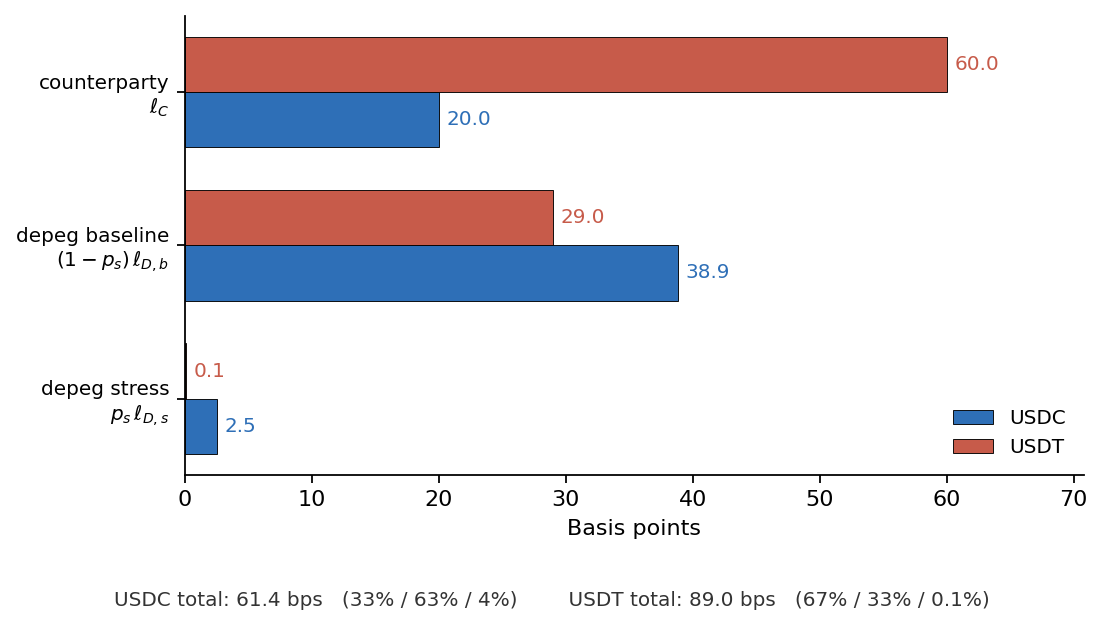
\includegraphics[width=0.85\textwidth]{fig_risk_decomposition.pdf}
\caption{The two decompositions side by side: USDC depeg-dominant, USDT counterparty-dominant.}\label{fig:decomp}
\end{figure}

\section{Comparing with other payment methods}\label{sec:empirical_comparison}

We carry each premium into a corridor-level cost comparison. A non-stablecoin rail costs $c=\phi+\kappa_W\tau$ (fee plus the working-capital cost of settlement delay); a stablecoin rail costs $c^{\text{stable}}=\phi+b_{\text{dest}}+\Pi_{\text{risk}}$, adding the destination off-ramp basis and the structural premium. Per-rail fees are RPW Q3 2025 means for the cross-border corridors and published schedules for the domestic rails. Three corridors span the policy-relevant space (Table~\ref{tab:uc_dt}).

\begin{table}[H]
\centering
\caption{Three corridors, total cost in basis points. Stablecoin $=$ USDT on corridors 1--2, USDC on corridor 3 (the realistic choice on each).}\label{tab:uc_dt}
\begin{tabular}{lrrrl}
\toprule
Corridor (amount) & Stablecoin & Wise & SWIFT & Public rail \\
\midrule
Brazil domestic (USD 40)    & 467.2 & --    & --    & PIX $=$ 0 \\
US--Mexico (USD 400)        & 120.7 & 251.2 & 333.5 & none yet \\
EU--Brazil (USD 1{,}000)    & 84.9  & 205.2 & 489.5 & none yet \\
\bottomrule
\end{tabular}
\end{table}

The three corridors trace three regimes.

\paragraph{Dominated where a public rail exists.}\label{sub:bra_domestic} On the Brazilian domestic corridor PIX clears at zero cost; the stablecoin is the most expensive rail at 467 basis points, because the flat on-chain fee dominates at a small ticket. An upgraded public rail that already exists wins outright.

\paragraph{Wins where none exists.} On US--Mexico, USDT at 121 basis points beats Wise by 130 and SWIFT by 213; the fintech-upgraded incumbent (Wise) is the closest competitor, and the residual gap is what the stablecoin captures.

\paragraph{Still wins cross-border, but with a sunset.}\label{sub:eu_br} On EU--Brazil, USDC at 85 basis points beats Wise by 120 and SWIFT by 405. But an upgraded public cross-border rail changes the ranking: a BIS Project Nexus rail \citep{bis_nexus_2024} priced at the SEPA-Instant level would cost about 5 basis points at USD 400 and 2 at USD 1{,}000, absorbing the stablecoin's advantage by two orders of magnitude. Where such a rail is under construction, the stablecoin's edge has a sunset matched to the public timetable.

\section{Policy reading}\label{sec:discussion}

\subsection{Implications for central banks}\label{sub:policy_implications}

Two points follow. First, \textbf{where it wins, the stablecoin is a bridge, not a frontier}: it fills a cross-border infrastructure gap that an interlinked public instant-payment system would otherwise fill at a fraction of the cost, so the build-versus-license decision is first-order, and the risk premium is a structural cost no operational improvement removes. Second, \textbf{the category is too coarse for one supervisory rule}: USDC's premium is depeg-dominant and USDT's counterparty-dominant, so a framework calibrated to one misprices the other. A prudential design with a liquidity-ratio and a capital-ratio instrument \citep{goel_lewrick_agarwal_2026} should be tilted toward secondary-market depth for USDC and toward reserve quality and capital for USDT. The decomposition is what makes such a framework issuer-specific rather than category-wide.

The comprehensive treatment, including the formal model and propositions, the calibration and identification diagnostics, the regulatory-uncertainty band, and the robustness analysis, is in the companion internet appendix.

\clearpage
\bibliographystyle{plainnat}
\bibliography{refs}

\clearpage
\appendix
\section{The model in brief}\label{app:dt_model}

\textbf{Primitives.} A unit mass of holders share an issuer fundamental $\theta$, drawn from a regime-dependent normal prior ($\rho\in\{b,s\}$, with $\mathbb{P}(\rho=s)=p_s$). The issuer redeems at par up to liquid reserves $R$; unmet demand $U(D)=\max\{D-R,0\}$ clears on a secondary market at
\[
p^{sec}(D)=\min\!\Big\{1,\ \max\big[\underline p,\ 1-\psi\,(U(D)/\widetilde M(D))^{\nu}-\mu_q q\big]\Big\},\qquad
\widetilde M(D)=\frac{M}{1+\zeta\,U(D)/M},
\]
with convex price impact ($\nu>1$) and stress-contracting depth ($\zeta$). The payoff to converting is $V_R(D)=\min\{1,R/D\}+(1-\min\{1,R/D\})\,p^{sec}(D)-\phi$ and to holding $V_H(\theta)=\theta-c_q q+\omega-\xi h$; the equilibrium threshold solves \eqref{eq:fixedpoint}.

\textbf{Properties (proved in the internet appendix).} Under a noisy signal and convex price impact the best-response map is a contraction, so the threshold is unique. A deeper reserve raises the anticipated secondary price and weakly raises conversion; a higher convenience yield $\omega$ lowers it. These are the comparative statics that make reserve quality and payment use primitives that move the priced premium.

\textbf{Calibration summary.} Seven free parameters $\phi=(\sigma,\psi,\nu,\mu_q,\zeta,\mu_s,\tau_s)$ are matched to six price moments per issuer by Nelder--Mead on a weighted loss. The converged vectors are $\phi^{\text{USDC}}=(0.194,0.275,1.741,0.053,0.507,0.212,9.88)$ at loss $1.82$ and $\phi^{\text{USDT}}=(0.237,0.108,4.000,0.022,0.453,0.231,7.98)$ at loss $0.16$, with $p_s=0.0108$. The decomposition of Table~\ref{tab:decomp} is computed at these vectors.

\end{document}
